\documentclass[a4paper,10pt, DIV=11]{scrartcl}
%\documentclass[a4paper,11pt,DIV=11,oneside]{scrreprt} % 
\usepackage[envcountsect]{beamerarticle}
\setjobnamebeamerversion{geometry.beamer}

%\documentclass[unknownkeysallowed]{beamer}

\usepackage[utf8]{inputenc}
\usepackage{lmodern}

\setcounter{tocdepth}{2}

\usepackage{listings}

% For For-Loops
\usepackage{forloop}
\newcounter{ct}

\usepackage{graphicx}
\usepackage{xcolor}
\usepackage{tikz}
\usetikzlibrary{arrows, snakes, backgrounds}
\usepackage{wrapfig}

\setbeamercovered{transparent}
% for \uptau
\usepackage{upgreek}

\title{Rate Monotonic vs. EDF: Judgment Day}
\subtitle{von Buttazzo, G. C.}
\date{\today}
\author{Dominik Schlecht}
\institute[THI]{Technische Hochschule Ingolstadt}

% Farben der THI
\definecolor{THIblue}{rgb}{0.0078,0.1176,0.4705}
%%-------------Allgemeine Definitionen----------------------------------
% Farbige Aufwertung der berschriften
%\addtokomafont{chapter}{\color{THIblue}}
\addtokomafont{section}{\color{THIblue}}
\addtokomafont{caption}{\color{THIblue}}
\addtokomafont{subsection}{\color{THIblue}}
\addtokomafont{subsubsection}{\color{THIblue}}
\setkomafont{captionlabel}{\color{THIblue}}

%Hyperref
\usepackage[
		pdftex,
		linkcolor=THIblue,			% Farbe der Verlinkung
		linktocpage=true,			% Im TOC wird Seitenzahl verlinkt(true),bzw. Text(false)
		colorlinks=true,			% 'true' keinen Kasten um Link
		citecolor=THIblue,
%		pdfhighlight=/P,
%		bookmarks,
%		hyperfigures=true,
%		citebordercolor={0 0 1},
%		linkbordercolor={0 0 1},
%		menubordercolor={0 0 1},
%		backref=true,
%		pagebackref=true,
%		bookmarksopen,
%		bookmarksnumbered,
%		pdfpagelabels=false,
%		pdfstartpage=1,
%		pdfstartview=Fit,			% Modus beim Öffnen (Fit = An Seitengröße anpassen)
		pdftitle={Rate Monotonics vs. Earliest Deadline First},
		pdfauthor={Dominik Schlecht},
%		pdfstartview=Fit,
%		pdfdisplaydoctitle=true,
%		plainpages=false
			]{hyperref} 
			
\usepackage{scrpage2} 	% Kopf & Fußzeile im KOMA Stil
\pagestyle{scrheadings}	% Aktiviert Verwendung vordefinierter Kolumnentitel
\clearscrheadfoot 		% alle Standard-Werte und Formatierungen löschen
\setkomafont{pagehead}{\scshape}	% Schriftart in Kopfzeile, \scshape = Kapitelchen
\automark[chapter]{section} % [linke Seite]{rechte Seite}
%\ohead{\def\pagestyle{PDTS}{\hrulefill\includegraphics[width = 6cm]{bilder/thi_logo_quer_cropped}}}
\ohead{\includegraphics[width = 5cm]{handout/bilder/thi_logo_quer_cropped}}

%\ihead{\textsc{Abschlussarbeit}}
%\ohead{\headmark}
\ihead{Rate Monotonics vs. Earliest Deadline First}

%\setheadwidth[0pt]{textwithmarginpar}
\ofoot{\vspace{-0.3cm} \pagemark} 						
\ifoot{\vspace{-0.3cm} Dominik Schlecht} 
				
%\setheadtopline{.4pt}				
\setheadsepline{.2pt}
\setfootsepline{.4pt}	% Trennlinie Fußzeile und Textkörper

% Document..
\begin{document}
	\frame{\maketitle}
	\frame{\tableofcontents[hideallsubsections]}
	\newpage
	
	\section{Einleitung}
	\subsection{Meta-Informationen}
\begin{frame}{\subsecname}
	\begin{itemize}
		\item Author:
		\begin{itemize}
			\item Giorgio C. Buttazzo
			\item University of Pavia, Italien
			\item buttazzo@unipv.it
		\end{itemize}
		\item Whitepaper
		\begin{itemize}
			\item Rate Monotonic vs. EDF: Judgment Day
			\item Real-Time Systems, 29, 5–26, 2005
		\end{itemize}						
		
	\end{itemize}
\end{frame} 

\subsection{Abstract}
\begin{frame}{\subsecname}
\tiny Since the first results published in 1973 by Liu and Layland on the Rate Monotonic (RM) and Earliest Deadline First (EDF) algorithms, a lot of progress has been made in the schedulability analysis of periodic task sets. Unfortunately, many misconceptions still exist about the properties of these two scheduling methods, which usually tend to favor RM more than EDF. Typical wrong statements often heard in technical conferences and even in research papers claim that RM is easier to analyze than EDF, it introduces less runtime overhead, it is more predictable in overload conditions, and causes less jitter in task execution.Since the above statements are either wrong, or not precise \tiny, it is time to clarify these issues in a systematic fashion, because the use of EDF allows a better exploitation of the available resources and significantly improves system’s performance. This paper compares RM against EDF under several aspects, using existing theoretical results, specific simulation experiments, or simple counterexamples to show that many common beliefs are either false or only restricted to specific situations.\footnote{Rate Monotonics vs. EDF: Judgment Day, Girorgio C. Buttazzo, 2005}
\end{frame}

\begin{frame}{\subsecname}
\includegraphics[width=\textwidth]{graphics/memes/aintnobody.jpg}
\end{frame}

\begin{frame}{\subsecname}
\tiny Since the first results published in 1973 by Liu and Layland on the Rate Monotonic (RM) and Earliest Deadline First (EDF) algorithms, a lot of progress has been made in the schedulability analysis of periodic task sets. Unfortunately, many \Large misconceptions \tiny still exist about the properties of these two scheduling methods, which usually tend to favor RM more than EDF. Typical wrong statements often heard in technical conferences and even in research papers claim that RM is easier to analyze than EDF, it introduces less runtime overhead, it is more predictable in overload conditions, and causes less jitter in task execution.Since the above statements are either wrong, or not precise, it is time to clarify these issues in a systematic fashion, because the use of EDF allows a better exploitation of the available resources and significantly improves system’s performance. This paper compares RM against EDF under several aspects, using existing theoretical results, specific simulation experiments, or simple counterexamples to show that many common beliefs are either false or only restricted to specific situations.\footnote{Rate Monotonics vs. EDF: Judgment Day, Girorgio C. Buttazzo, 2005}
\end{frame}
	
\begin{frame}{\subsecname}
\tiny Since the first results published in 1973 by Liu and Layland on the Rate Monotonic (RM) and Earliest Deadline First (EDF) algorithms, a lot of progress has been made in the schedulability analysis of periodic task sets. Unfortunately, many \Large misconceptions \tiny still exist about the properties of these two scheduling methods, which usually tend to \Large favor RM more than EDF \tiny. Typical wrong statements often heard in technical conferences and even in research papers claim that RM is easier to analyze than EDF, it introduces less runtime overhead, it is more predictable in overload conditions, and causes less jitter in task execution.Since the above statements are either wrong, or not precise, it is time to clarify these issues in a systematic fashion, because the use of EDF allows a better exploitation of the available resources and significantly improves system’s performance. This paper compares RM against EDF under several aspects, using existing theoretical results, specific simulation experiments, or simple counterexamples to show that many common beliefs are either false or only restricted to specific situations.\footnote{Rate Monotonics vs. EDF: Judgment Day, Girorgio C. Buttazzo, 2005}
\end{frame}

	\begin{frame}{\subsecname}
\tiny Since the first results published in 1973 by Liu and Layland on the Rate Monotonic (RM) and Earliest Deadline First (EDF) algorithms, a lot of progress has been made in the schedulability analysis of periodic task sets. Unfortunately, many \Large misconceptions \tiny still exist about the properties of these two scheduling methods, which usually tend to \Large favor RM more than EDF \tiny. Typical wrong statements often heard in technical conferences and even in research papers claim that RM is easier to analyze than EDF, it introduces less runtime overhead, it is more predictable in overload conditions, and causes less jitter in task execution.Since the above statements are \Large  either wrong, or not precise \tiny, it is time to clarify these issues in a systematic fashion, because the use of EDF allows a better exploitation of the available resources and significantly improves system’s performance. This paper compares RM against EDF under several aspects, using existing theoretical results, specific simulation experiments, or simple counterexamples to show that many common beliefs are either false or only restricted to specific situations.\footnote{Rate Monotonics vs. EDF: Judgment Day, Girorgio C. Buttazzo, 2005}
\end{frame}
	
\begin{frame}{\subsecname}
\tiny Since the first results published in 1973 by Liu and Layland on the Rate Monotonic (RM) and Earliest Deadline First (EDF) algorithms, a lot of progress has been made in the schedulability analysis of periodic task sets. Unfortunately, many \Large misconceptions \tiny still exist about the properties of these two scheduling methods, which usually tend to \Large favor RM more than EDF \tiny. Typical wrong statements often heard in technical conferences and even in research papers claim that RM is easier to analyze than EDF, it introduces less runtime overhead, it is more predictable in overload conditions, and causes less jitter in task execution.Since the above statements are \Large  either wrong, or not precise \tiny, it is time to clarify these issues in a systematic fashion, because the use of EDF allows a better exploitation of the available resources and significantly improves system’s performance. \Large This paper compares RM against EDF \tiny under several aspects, using existing theoretical results, specific simulation experiments, or simple counterexamples to show that many common beliefs are either false or only restricted to specific situations.\footnote{Rate Monotonics vs. EDF: Judgment Day, Girorgio C. Buttazzo, 2005}
\end{frame}


\begin{frame}{\subsecname}
	\begin{center}
		\includegraphics[scale=0.6]{graphics/memes/mythbusters_thisweek.jpg}
	\end{center}
\end{frame}

%\section{Erläuterung}
\subsection{Flashback - Scheduling}
\begin{frame}{\subsecname}
	Wir definieren:
	\begin{equation}
		\uptau_{i, k} \text{ als Job mit einer absoluten Deadline } d_{i, k}
	\end{equation}
	\pause
	\begin{equation}
		\uptau_i \text{ als infinite Folge von Jobs } \uptau_{i, k} \text{ mit }
	\end{equation}
	\pause
	\begin{equation}
		\begin{array}{l l l}
			\text{Wort-Case-Execution-Time } & C_i\\
			\text{Task-Period } & T_i
		\end{array}
	\end{equation}
\end{frame}

\begin{frame}
	Klartext:\\
	\begin{center}
		%\rowcolors{1}{RoyalBlue!20}{RoyalBlue!5}
		\begin{tabular}{c||c|c}
			Task ($\uptau_i$) & Dauer ($C_i$) & Task-Periode ($T_i$)\\\hline\hline
			$\uptau_i$ & 5 & 15
		\end{tabular}
	\end{center}
\end{frame}

\begin{frame}
	\input{graphics/einleitung/simple1.tex}
\end{frame}

\begin{frame}
	\begin{figure}[htbp]
	% Partly taken from http://www.texample.net/tikz/examples/convolution-of-two-functions/
	\centering
	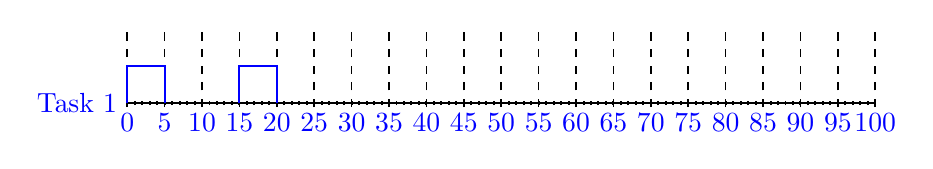
\begin{tikzpicture}[
		scale=0.095,
		line width=0.25mm,
		every node/.style={scale=1, text=blue},
		major tick/.style={semithick, dashed},
		x tick label/.style={anchor=north, minimum width=5mm},
		task1/.style={blue},
		task2/.style={red},
		task3/.style={green},
		desc/.style={anchor=east}
		]
	
	% Task 1
	\draw (0, 0) -- (100, 0);
	\node[desc] at (0, 0) {Task 1};
	
%	% Task 2
%	\draw (0, 10) -- (100, 10);
%	\node[desc] at (0, 10) {Task 2};	
%	
%	% Task 3
%	\draw (0, 20) -- (100, 20);
%	\node[desc] at (0, 20) {Task 3};	
	
	% Small ticks
	\foreach \x in {0, 1,...,100}{
		\draw (\x, -0.25) -- (\x, 0.25);
	}
	
	% Major ticks with label
	\foreach \x/\label in {0, 5,...,100}{
		\node[x tick label] at (\x, 0) {$\label$}; 		
		\draw[major tick] (\x, -0.5) -- (\x, 10);
	}
	
	% Draw all
%	\foreach \x in {0, 15,...,100}{
%		\draw[task1] (\x, 0) -- (\x, 5) -- (\x+5, 5) -- (\x+5, 0);
%	}
	
	% Single steps for the slides
	\draw[task1] (0, 0) -- (0, 5) -- (5, 5) -- (5, 0);
	\draw[task1] (15, 0) -- (15, 5) -- (20, 5) -- (20, 0);
%	\draw[task1] (30, 0) -- (30, 5) -- (35, 5) -- (35, 0);
%	\draw[task1] (45, 0) -- (45, 5) -- (50, 5) -- (50, 0);
%	\draw[task1] (60, 0) -- (60, 5) -- (65, 5) -- (65, 0);
%	\draw[task1] (75, 0) -- (75, 5) -- (80, 5) -- (80, 0);
%	\draw[task1] (90, 0) -- (90, 5) -- (95, 5) -- (95, 0);

	\end{tikzpicture}
\end{figure}
\end{frame}

\begin{frame}
	\begin{figure}[htbp]
	% Partly taken from http://www.texample.net/tikz/examples/convolution-of-two-functions/
	\centering
	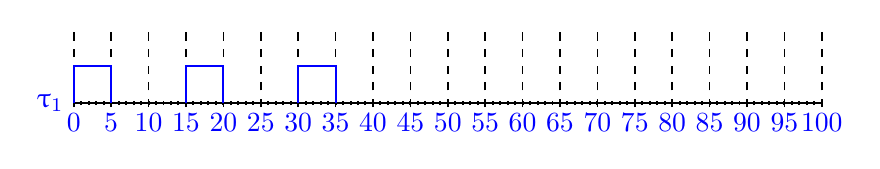
\begin{tikzpicture}[
		scale=0.095,
		line width=0.25mm,
		every node/.style={scale=1, text=blue},
		major tick/.style={semithick, dashed},
		x tick label/.style={anchor=north, minimum width=5mm},
		task1/.style={blue},
		task2/.style={red},
		task3/.style={green},
		desc/.style={anchor=east}
		]
	
	% Task 1
	\draw (0, 0) -- (100, 0);
	\node[desc] at (0, 0) {$\uptau_1$};
	
	\foreach \x in {0, 1,...,100}{
		\draw (\x, -0.25) -- (\x, 0.25);
	}
	
	% Major ticks with label
	\foreach \x/\label in {0, 5,...,100}{
		\node[x tick label] at (\x, 0) {$\label$}; 		
		\draw[major tick] (\x, -0.5) -- (\x, 10);
	}
	
	
	% Single steps for the slides
	\draw[task1] (0, 0) -- (0, 5) -- (5, 5) -- (5, 0);
	\draw[task1] (15, 0) -- (15, 5) -- (20, 5) -- (20, 0);
	\draw[task1] (30, 0) -- (30, 5) -- (35, 5) -- (35, 0);

	\end{tikzpicture}
\end{figure}
\end{frame}

\begin{frame}
	\input{graphics/einleitung/simple4.tex}
\end{frame}

\begin{frame}
	2 Tasks:
	\begin{center}
		\begin{tabular}{c||c|c}
				Task ($\uptau_i$) & Dauer ($C_i$) & Task-Periode ($T_i$)\\\hline\hline
				$\uptau_1$ & 5 & 15\\
				$\uptau_2$ & 10 & 40\\
		\end{tabular}
	\end{center}
\end{frame}

\begin{frame}
	\begin{figure}[htbp]
	% Partly taken from http://www.texample.net/tikz/examples/convolution-of-two-functions/
	\centering
	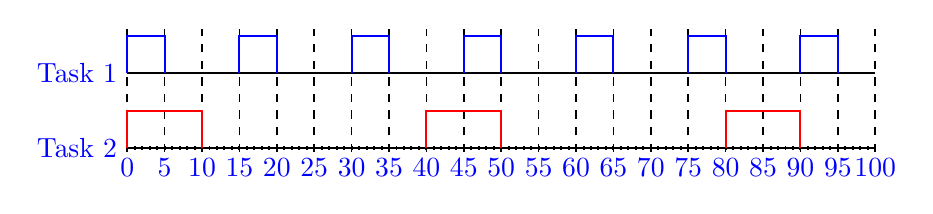
\begin{tikzpicture}[
		scale=0.095,
		line width=0.25mm,
		every node/.style={scale=1, text=blue},
		major tick/.style={semithick, dashed},
		x tick label/.style={anchor=north, minimum width=5mm},
		task1/.style={blue},
		task2/.style={red},
		task3/.style={green},
		desc/.style={anchor=east}
		]

	% Task 1
	\draw (0, 10) -- (100, 10);
	\node[desc] at (0, 10) {Task 1};
	
	% Task 2
	\draw (0, 0) -- (100, 0);
	\node[desc] at (0, 0) {Task 2};	
	
	% Small ticks
	\foreach \x in {0, 1,...,100}{
		\draw (\x, -0.25) -- (\x, 0.25);
	}
	
	% Major ticks with label
	\foreach \x/\label in {0, 5,...,100}{
		\node[x tick label] at (\x, 0) {$\label$}; 		
		\draw[major tick] (\x, -0.5) -- (\x, 16);
	}
	
	% Draw all Task 1
	\foreach \x in {0, 15,...,100}{
		\draw[task1] (\x, 10) -- (\x, 15) -- (\x+5, 15) -- (\x+5, 10);
	}
	
	% Draw all Task 2
	\foreach \x in {0, 40,...,100}{
		\draw[task2] (\x, 0) -- (\x, 5) -- (\x+10, 5) -- (\x+10, 0);
	}
	
	\end{tikzpicture}
\end{figure}
\end{frame}

\begin{frame}
	\begin{figure}[htbp]
	% Partly taken from http://www.texample.net/tikz/examples/convolution-of-two-functions/
	\centering
	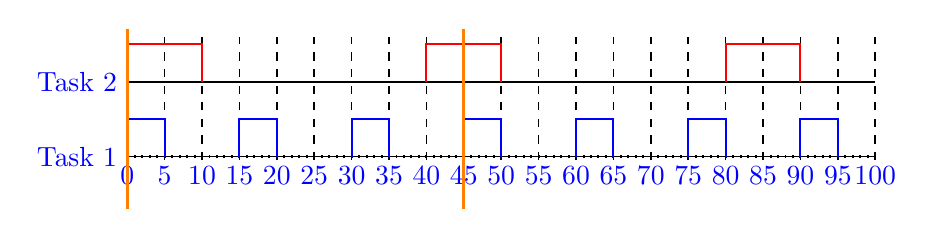
\begin{tikzpicture}[
		scale=0.095,
		line width=0.25mm,
		every node/.style={scale=1, text=blue},
		major tick/.style={semithick, dashed},
		x tick label/.style={anchor=north, minimum width=5mm},
		task1/.style={blue},
		task2/.style={red},
		task3/.style={green},
		desc/.style={anchor=east},
		konf/.style={orange, very thick}
		]
	
	% Task 1
	\draw (0, 0) -- (100, 0);
	\node[desc] at (0, 0) {Task 1};
	
	% Task 2
	\draw (0, 10) -- (100, 10);
	\node[desc] at (0, 10) {Task 2};	
%	
%	% Task 3
%	\draw (0, 20) -- (100, 20);
%	\node[desc] at (0, 20) {Task 3};	
	
	% Small ticks
	\foreach \x in {0, 1,...,100}{
		\draw (\x, -0.25) -- (\x, 0.25);
	}
	
	% Major ticks with label
	\foreach \x/\label in {0, 5,...,100}{
		\node[x tick label] at (\x, 0) {$\label$}; 		
		\draw[major tick] (\x, -0.5) -- (\x, 16);
	}
	
	% Draw all
	\foreach \x in {0, 15,...,100}{
		\draw[task1] (\x, 0) -- (\x, 5) -- (\x+5, 5) -- (\x+5, 0);
	}
	
	% Draw all
	\foreach \x in {0, 40,...,100}{
		\draw[task2] (\x, 10) -- (\x, 15) -- (\x+10, 15) -- (\x+10, 10);
	}
	
	\draw[konf] (0, 17) -- (0, -7);
	\draw[konf] (45, 17) -- (45, -7);
	
	\end{tikzpicture}
\end{figure}
\end{frame}

	
	\section{Rate Monotonic \& Earliest Deadline First}
	\subsection{Grundlagen}
\begin{frame}{\subsecname}
		\begin{columns}[]
  			\begin{column}{0.5\textwidth}
				Rate Monotonics:
				\begin{itemize}
					\item Task $T_i$ mit kürzester Periode wird bevorzugt
					\item Task $T_i$ wird anfangs eine Priorität zugewiesen
				\end{itemize}

			\end{column}
  			\begin{column}{0.5\textwidth}
  				Erliest Deadline First:
				\begin{itemize}
					\item Job $T_{i, k}$ mit der nächsten Deadline wird bevorzugt
					\item In diesem Paper ist die Deadline gleich mit der Periode
					\item Die Priorität von Task $T_i$ entscheidet sich während der Laufzeit
				\end{itemize}	
  			\end{column}
		\end{columns}
\end{frame}

\subsection{Beispiele}

\newcommand{\showRMSlide}[1] {\begin{frame}{Beispiel Rate Monotonics}
	\begin{center}
		\begin{tabular}{l||c|c}
				Task ($\uptau_i$) & Dauer ($C_i$) & Task-Periode ($T_i$)\\\hline\hline
				$\uptau_1$ & 4 & 10\\
				$\uptau_2$ & 2 & 16\\
				$\uptau_3$ & 8 & 20\\
		\end{tabular}
	\end{center}
	\input{graphics/rm/rm#1.tex}
\end{frame}}

\forloop{ct}{0}{\value{ct} < 11}%
{%
	\showRMSlide{\arabic{ct}}
}

\newcommand{\showEDFSlide}[1] {\begin{frame}{Beispiel Erliest Deadline First}
	\begin{center}
		\begin{tabular}{l||c|c}
				Task ($\uptau_i$) & Dauer ($C_i$) & Task-Periode ($T_i$)\\\hline\hline
				$\uptau_1$ & 4 & 10\\
				$\uptau_2$ & 2 & 16\\
				$\uptau_3$ & 8 & 20\\
		\end{tabular}
	\end{center}
	\input{graphics/edf/edf#1.tex}
\end{frame}}

\forloop{ct}{1}{\value{ct} < 14}%
{%
	\showEDFSlide{\arabic{ct}}
}
	
	\section{Vergleich}
	\subsection{Implementation Complexity}\label{ImplementationComplexity}
\begin{frame}{Mythos:}
	\begin{itemize}
		\item Rate Monotonics ist einfacher zu implementieren als Erliest Deadline First.
	\end{itemize}
\end{frame}

\begin{frame}{Fakt:}
	\begin{itemize}
		\item Auf einem kommerziellen Kernel mit festen Prioritätsleveln ist Rate Monotonics einfacher zu implementieren.
	\end{itemize}
\end{frame}
\begin{frame}{Weitere Faktoren:}
	\begin{itemize}
		\item Wird auf einem bestehenden System entwickelt?
		\item Sind die Prioritäten festgesetzt oder können diese während der Laufzeit verändert werden?
		\item Wie viele Prioritäts-Level gibt es?
	\end{itemize}
\end{frame}

\begin{frame}{Annahme:}
	\begin{itemize}
		\item Das System wird von Grund auf mit einer Ready-Queue implementiert.\pause
		\item In dieser werden die Tasks für Rate Monotonics
			\begin{itemize}
				\item absteigend nach nach dem Prioritäten-Level
			\end{itemize}
			und für Erliest Deadline First
			\begin{itemize}
				\item aufsteigend nach der absoluten Deadline
			\end{itemize} gespeichert.
	\end{itemize}
\end{frame}

\begin{frame}{Fazit:}
	\begin{itemize}
		\item Unter den richtigen Vorbedingungen ist auch EDF leicht zu implementieren.
	\end{itemize}
\end{frame}


\subsection{Runtime Overhead}\label{RuntimeOverhead}
\begin{frame}{Mythos:}
	\begin{itemize}
		\item Rate Monotonics produziert weniger Runtime-Overhead, da die Prioritäten währen der Laufzeit nicht neu berechnet werden müssen.
	\end{itemize}
\end{frame}

\begin{frame}{Beispiel}
	\begin{center}
		\begin{tabular}{c||c|c}
			Task ($\uptau_i$) & Dauer ($C_i$) & Task-Periode ($T_i$)\\\hline\hline
			$\uptau_1$ & 4 & 10\\
			$\uptau_2$ & 8 & 14
		\end{tabular}
	\end{center}
	\begin{itemize}
		\item Rate Monotonics:
	\end{itemize}
	\input{graphics/vergleich/runtimeOverhead7_RM.tex}
	\begin{itemize}
		\item Earliest Deadline First:	
	\end{itemize}

	\input{graphics/vergleich/runtimeOverhead1_EDF.tex}
\end{frame}

\begin{frame}{Context-Switching/Preemptions:}
	\begin{itemize}
		\item Umschalten zwischen verschiedenen Tasks.
		\item Zieht Aufwände mit sich.
	\end{itemize}
\end{frame}

\newpage
\begin{frame}{Vergleich Rate Monotonics vs. Earliest Deadline First}
	\begin{itemize}
		\item Rate Monotonics:
	\end{itemize}
	\input{graphics/vergleich/runtimeOverhead_RM_C.tex}
	\begin{itemize}
		\item Earliest Deadline First:	
	\end{itemize}
	\begin{figure}[htbp]
	% Partly taken from http://www.texample.net/tikz/examples/convolution-of-two-functions/
	\centering
	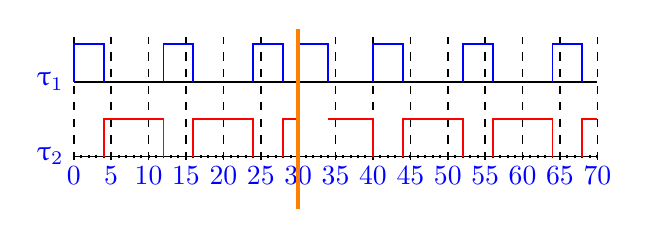
\begin{tikzpicture}[
		scale=0.095,
		line width=0.25mm,
		every node/.style={scale=1, text=blue},
		major tick/.style={semithick, dashed},
		x tick label/.style={anchor=north, minimum width=5mm},
		task1/.style={blue},
		task2/.style={red},
		task3/.style={green},
		desc/.style={anchor=east},
		konf/.style={orange, very thick}
		]
	
	% Task 2
	\draw (0, 0) -- (70, 0);
	\node[desc] at (0, 0) {$\uptau_2$};
	
	% Task 1
	\draw (0, 10) -- (70, 10);
	\node[desc] at (0, 10) {$\uptau_1$};	
	
	% Small ticks
	\foreach \x in {0, 1,...,70}{
		\draw (\x, -0.25) -- (\x, 0.25);
	}
	
	% Major ticks with label
	\foreach \x/\label in {0, 5,...,70}{
		\node[x tick label] at (\x, 0) {$\label$}; 		
		\draw[major tick] (\x, -0.5) -- (\x, 16);
	}
	
	% Draw all
%	\foreach \x in {0, 10,...,69}{
%		\draw[task1] (\x, 10) -- (\x, 15) -- (\x+4, 15) -- (\x+4, 10);
%	}

	\draw[task1] (0, 10) --  (0, 15) --  (4, 15) -- (4, 10);
	\draw[task2] (4, 0) --  (4, 5) --  (12, 5) -- (12, 0);
	\draw[task1] (12, 10) --  (12, 15) --  (16, 15) -- (16, 10);
	\draw[task2] (16, 0) --  (16, 5) --  (24, 5) -- (24, 0);
	\draw[task1] (24, 10) --  (24, 15) --  (28, 15) -- (28, 10);
	\draw[task2] (28, 0) --  (28, 5) --  (30, 5); % 2 done
	\draw[task1] (30, 10) --  (30, 15) --  (34, 15) -- (34, 10);
	\draw[task2] (34, 5) --  (40, 5) -- (40, 0);	
	\draw[task1] (40, 10) --  (40, 15) --  (44, 15) -- (44, 10);
	\draw[task2] (44, 0) --  (44, 5) --  (52, 5) -- (52, 0);
	\draw[task1] (52, 10) --  (52, 15) --  (56, 15) -- (56, 10);
	\draw[task2] (56, 0) --  (56, 5) --  (64, 5) -- (64, 0);
	\draw[task1] (64, 10) --  (64, 15) --  (68, 15) -- (68, 10);
	\draw[task2] (68, 0) --  (68, 5) --  (70, 5);
	
	\draw[konf] (30, 17) -- (30, -7);	
	
	\end{tikzpicture}
%	\caption{Ablaufübersicht}
\end{figure} 
\end{frame}

\begin{frame}{Fazit:}
	\begin{itemize}
		\item Beachtet man den Aufwand der Context-Switches, erzeugt Rate Monotonics mehr Overhead als Earliest Deadline First
	\end{itemize}
\end{frame}


\subsection{Schedulability Analysis}\label{SchedulabilityAnalaysis}
\begin{frame}{Erklärung:}
	Schedulability meint, dass eine Menge von periodischen Task mithilfe eines Algorithmus planbar ist.
\end{frame}
\begin{frame}{Mythos:}
	\begin{itemize}
		\item Die Einteilung ist bei Rate Monotonics leichter berechenbar als bei Erliest Deadline First.
	\end{itemize}
\end{frame}

\begin{frame}{Allgemein gilt:}
	
	\begin{equation}
		U_i = C_i / T_i
	\end{equation}
	Desweiteren gilt, dass ein Task-Set $P$ unter RM nur sicher planbar seien kann, wenn
	\begin{equation}
		\prod_{i=0}^n (U_i +1) \leq 2
	\end{equation}
	und unter EDF nur (und auch wirklich nur) planbar sein, wenn
	\begin{equation}
		\sum_{i=1}^n U_i \leq 1
	\end{equation}
\end{frame}

\begin{frame}{Beispiel:}
	\begin{center}
		\begin{tabular}{c||c|c}
			Task ($\uptau_i$) & Dauer ($C_i$) & Task-Periode ($T_i$)\\\hline\hline
			$\uptau_1$ & 1 & 4\\
			$\uptau_2$ & 3 & 8\\
			$\uptau_3$ & 2 & 16
		\end{tabular}	
		\begin{itemize}
			\item RM: $U = (\frac{1}{4}+1)(\frac{3}{8}+1)(\frac{2}{16}+1)\approx 1.93 \leq 2$
			\item EDF: $U = \frac{1}{4} + \frac{3}{8} + \frac{2}{16} = \frac{3}{4} = 0.75 \leq 1$
		\end{itemize}
	\end{center}

\end{frame}

\begin{frame}

\end{frame}

\begin{frame}{RTA und PDC}
	Response Time Analysis (RTA) Algorithmus für Rate Monotonics:
	\begin{equation}
		D_i \geq
		\begin{cases}
   				R_i^{(0)}=C_i \\
   				R_i^{(k)}=C_i+ \sum_{j:D_j<D_i} \lceil \frac{R_i^{k-1}}{T_j}\rceil C_j
  		\end{cases}
	\end{equation}
	Processor Demand Criterion (PDC) Algorithmus für Erliest Deadline First:
	\begin{equation}
		\forall L > 0,\; \sum_{i=1}^n\lfloor \frac{L+T_i-D_i}{T_i}\rfloor C_i \leq L
	\end{equation}

	\begin{figure}[htbp]
		\begin{center}	
			\includegraphics[scale=.30]{graphics/vergleich/rtapdc.png}
		\end{center}
		\caption{Vergleich RTA vs. PDC \footnote{Rate Monotonics vs. EDF: Judgment Day, Girorgio C. Buttazzo, 2005}}	
		\label{fig:RTAvsPDC}
	\end{figure}
\end{frame}

\newpage
\begin{frame}{Fazit:}
	\begin{itemize}
		\item Komplexität für Rate Monotonics: pseudo-polynomial
		\item Komplexität für Erliest Deadline First:
		\begin{itemize}
			\item pseudo-polynomial
			\item in besonderen Fällen $O(n)$
		\end{itemize}
		\item Bei einer hohen Anzahl von Tasks ist Rate Monotonics besser zu berechnen (siehe Figure \ref{fig:RTAvsPDC} auf Seite \pageref{fig:RTAvsPDC}).
		\item Bei Erliest Deadline First ist für höhere Auslastungen ein garantiertes Scheduling möglich.
	\end{itemize}
\end{frame}

\subsection{Robustness During Overloads}\label{RobustnessDuringOverloads}

\begin{frame}{Mythos:}
	\begin{itemize}
		\item Rate Monotonics ist in Overload-Situationen besser vorhersehbar.
	\end{itemize}
\end{frame}

\subsubsection{Permanent Overload}
\begin{frame}{Permanent Overload: Taskset}
	\begin{center}
		\begin{tabular}{c||c|c}
			Task ($\uptau_i$) & Dauer ($C_i$) & Task-Periode ($T_i$)\\\hline\hline
			$\uptau_1$ & 4 & 8\\
			$\uptau_2$ & 6 & 12\\
			$\uptau_3$ & 5 & 20
		\end{tabular}
		
	\end{center}
\end{frame}

\begin{frame}{Permanent Overload: Rate Monotonics}
\begin{itemize}
			\item $U=(\frac{4}{8}+1)(\frac{6}{12}+1)(\frac{5}{20}+1)\approx 2.81 \nleq 2$\pause		
		\end{itemize}				

		\begin{figure}[htbp]
	% Partly taken from http://www.texample.net/tikz/examples/convolution-of-two-functions/
	\centering
	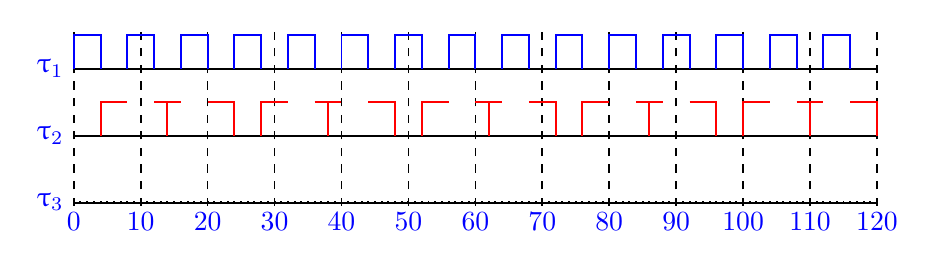
\begin{tikzpicture}[
		scale=0.085,
		line width=0.25mm,
		every node/.style={scale=1, text=blue},
		major tick/.style={semithick, dashed},
		x tick label/.style={anchor=north, minimum width=5mm},
		task1/.style={blue},
		task2/.style={red},
		task3/.style={green},
		desc/.style={anchor=east}
		]


	% Task 3
	\draw (0, 0) -- (120, 0);
	\node[desc] at (0, 0) {$\uptau_3$};
	
	% Task 2
	\draw (0, 10) -- (120, 10);
	\node[desc] at (0, 10) {$\uptau_2$};	

	% Task 1
	\draw (0, 20) -- (120, 20);
	\node[desc] at (0, 20) {$\uptau_1$};	

	
	% Small ticks
	\foreach \x in {0, 1,...,120}{
		\draw (\x, -0.25) -- (\x, 0.25);
	}
	
	% Major ticks with label
	\foreach \x/\label in {0, 10,...,120}{
		\node[x tick label] at (\x, 0) {$\label$}; 		
		\draw[major tick] (\x, -0.5) -- (\x, 26);
	}
	
	% Draw all
	\foreach \x in {0, 24,...,100}{
		\draw[task1] (\x, 20) -- (\x, 25) -- (\x+4, 25) -- (\x+4, 20);
		\draw[task2] (\x+4, 10) -- (\x+4, 15) -- (\x+8, 15);
		\draw[task1] (\x+8, 20) -- (\x+8, 25) -- (\x+12, 25) -- (\x+12, 20);
		\draw[task2] (\x+12, 15) -- (\x+14, 15) -- (\x+14, 10);
		\draw[task2] (\x+14, 10) -- (\x+14, 15) -- (\x+16, 15);
		\draw[task1] (\x+16, 20) -- (\x+16, 25) -- (\x+20, 25) -- (\x+20, 20);
		\draw[task2] (\x+20, 15) -- (\x+24, 15) -- (\x+24, 10);
	}

%	\draw[task1] (0, 10) --  (0, 15) --  (4, 15) -- (4, 10);	

		
	\end{tikzpicture}
%	\caption{Ablaufübersicht}
\end{figure} 
\end{frame}

\begin{frame}{Permanent Overload: Erliest Deadline First}
	\begin{center}
		\begin{itemize}
			\item $U=\frac{4}{8}+\frac{6}{12}+\frac{5}{20}=1.25 \nleq 1$\pause		
		\end{itemize}

	\input{graphics/vergleich/robustness1_EDF.tex}
	\end{center}
\end{frame}

\begin{frame}{Vergleich Permanent Overload}
	\begin{columns}[]
  			\begin{column}{0.5\textwidth}
				Rate Monotonics:
				\begin{itemize}
					\item Tasks mit langer Periode werden vollständig blockiert!
					\item Gut vorhersagbar.
				\end{itemize}

			\end{column}
  			\begin{column}{0.5\textwidth}
  				Erliest Deadline First:
				\begin{itemize}
					\item Sieht chaotischer aus.
					\item Durchschnittliche Periode $\bar{T}_i$ für einen Task $\uptau_i$ ist gegeben durch
						\begin{equation}
							\bar{T}_i=T_i\cdot U
						\end{equation}
				\end{itemize}	
  			\end{column}
	\end{columns}
\end{frame}

%\begin{frame}{\subsubsecname}
%	Beispiel mit EDF? %TODO
%\end{frame}

\begin{frame}{Fazit Permanent Overload:}
	
	\begin{itemize}
		\item Beide Verfahren bei permanenter Überlastung gut vorhersagbar.
		\item Einsatzgebiet ist stark Situationsabhängig.
	\end{itemize}
\end{frame}

\subsubsection{Transient Overload}
\begin{frame}{Annahme für Rate Monotonics:}
	\begin{itemize}
		\item Es werden Tasks mit kurzen Perioden bevorzugt.\pause
		\item[$\Rightarrow$] Falls ein Task seine Deadline überschreitet, wird der Task mit der längsten Periodenlänge verschoben/unterbrochen	.
	\end{itemize}
\end{frame}

\newcommand{\showRMSlideRob}[1] {\begin{frame}{Gegenbeispiel}
	\begin{center}
		\begin{tabular}{c||c|c}
			Task ($\uptau_i$) & Dauer ($C_i$) & Task-Periode ($T_i$)\\\hline\hline
			$\uptau_1$ & 6 & 15\\
			$\uptau_2$ & 9 & 27\\
			$\uptau_3$ & 3 & 60\\
			$\uptau_4$ & 3 & 90
		\end{tabular}
	\end{center}
	\input{graphics/vergleich/transient#1_RM.tex}
	
	\begin{itemize}
		\item[$\Rightarrow$] $\uptau_2$ wird unterbrochen, während Task $\uptau_3$ und $\uptau_4$ nicht beeinflusst werden!
	\end{itemize}
\end{frame}}

\forloop{ct}{7}{\value{ct} < 8}%
{%
	\showRMSlideRob{\arabic{ct}}
}


\begin{frame}{Fazit:}
	\begin{itemize}
		\item Permanent Overload: Gleichwertig.
		\item Transient Overload:
		\begin{itemize}
			\item Rate Monotonics verführt zu falschen Annahmen.
		\end{itemize}
	\end{itemize}
\end{frame}


\subsection{Jitter and Latency}\label{JitterandLatency}

\begin{frame}{Absolute Response Time Jitter}
	Absolute Response Time Jitter $ARJ_i$ ist definiert durch
	\begin{equation}
		ARJ_i=max R_{i,k}-min R_{i,k}
	\end{equation} mit
	$R_{i,K}$ als Response-Time für den $k$-ten Job von $\uptau_i$.
\end{frame}

\begin{frame}{Mythos:}
	\begin{itemize}
		\item Durch die festen Prioritäten entsteht währen der Laufzeit bei Rate Monotonics weniger Jitter als bei Erliest Deadline First. 
	\end{itemize}
\end{frame}

\begin{frame}{Beispiel Taskset}
	\begin{center}
		\begin{tabular}{c||c|c}
			Task ($\uptau_i$) & Dauer ($C_i$) & Task-Periode ($T_i$)\\\hline\hline
			$\uptau_1$ & 2 & 6\\
			$\uptau_2$ & 3 & 8\\
			$\uptau_3$ & 2 & 12
		\end{tabular}	
	\end{center}
\end{frame}

\begin{frame}{Beispiel Jitter Rate Monotonics}
	\input{graphics/vergleich/jitter7_RM.tex}
\end{frame}

\begin{frame}{Beispiel Jitter Erliest Deadline First}
	\input{graphics/vergleich/jitter1_EDF.tex}
\end{frame}

\begin{frame}{\subsecname}
	\begin{figure}[htbp]
		\begin{center}
			\includegraphics[scale=.30]{graphics/vergleich/jitter.png}
		\end{center}
		\caption{Vergleich ARJ bei RM vs EDF\footnote{Rate Monotonics vs. EDF: Judgment Day, Girorgio C. Buttazzo, 2005}}
		\label{fig:jitter}
	\end{figure}
	
\end{frame}

\begin{frame}{Fazit:}
	\begin{itemize}
		\item RM hält Jitter für die hoch priorisierten Tasks sehr niedrig, vernachlässigt jedoch die anderen Tasks.
		\item Insgesamt erzeugt EDF, gerade bei hoher Auslastung, wesentlich weniger Jitter (siehe Figure \ref{fig:jitter} auf Seite \pageref{fig:jitter}).
	\end{itemize}
\end{frame}

%\subsection{Other Issues}
\subsubsection{Ressource Sharing}
\begin{frame}{\subsubsecname}
	Vorurteil:
	\begin{itemize}
		\item Es gibt nur für Rate Monotonics Protokolle um Zugriffe auf kritische Ressourcen zu regeln.
	\end{itemize}\pause
	Aber:
	\begin{itemize}
		\item Auch unter Erliest Deadline First gibt es diverse Algorithmen.
	\end{itemize}
\end{frame}

\subsubsection{Aperiodic Task Handling}
\begin{frame}{\subsubsecname}
	Test
\end{frame}

\subsubsection{Ressource Reservation}
\begin{frame}{\subsubsecname}
	Test
\end{frame}
	
	\newpage
	\section{Fazit}

	\begin{frame}<beamer>
		\frametitle{Gliederung}
		\tableofcontents[
  			currentsection,
  			sectionstyle=show/show,
  			subsectionstyle=show/shaded/hide,
  			squeeze
		]
	\end{frame}	
	
	\begin{frame}{Vorteile von Rate Monotonics:}
	\begin{itemize}
		\item leichtere Implementierung in kommerziellen Systemen
		\item RTA benötigt weniger Schritte als PDC
	\end{itemize}
\end{frame}

\begin{frame}{Vorteile Earliest Deadline First:}
	\begin{itemize}
		\item Erlaubt vertrauenswürdiges Scheduling solange $U \leq 1$
		\item Weniger Runtime Overhead
	\end{itemize}
\end{frame}

\begin{frame}{Unentschieden oder Situationsabhängig:}
	\begin{itemize}
		\item Overload Situations
		\item Jitter Control
	\end{itemize}
\end{frame}
Dies Zeigt, dass Rate Monotonics Earliest Deadline First nicht überlegen ist.
		
\end{document}